% ============================================================================
\section{Proposed System}
\label{sec:system}
% ============================================================================
The system separates two paths that meet in the knowledge base (Fig.~\ref{fig:architecture}). The update path runs when a regulation or company policy is issued and is the only path that uses a language model. The computation path runs at every payroll calculation and is deterministic. The figure marks the language model in orange, deterministic code in blue, and the human decision in green. One installation serves one company and holds only the policies of that company in its company layer. Every installation starts from the same validated regulation layer and keeps it current through its own updates.

\begin{figure*}[!t]
\centering
\figArchitecture
\caption{System architecture with the update path above and the computation path below.}
\label{fig:architecture}
\end{figure*}

\subsection{Two-Layer Bitemporal Knowledge Base}
\label{sec:representation}
The knowledge base is an RDF and OWL knowledge graph with SHACL validation and SPARQL queries. It holds documents, provisions, quotes, rules, parameters, tables, company policies, change events, and updates. The ontology reuses the European Legislation Identifier for documents and provisions~\cite{publicationsoffice2026elien}, OWL-Time for validity intervals~\cite{cox2017owltime}, and PROV-O for the update that generated each element~\cite{lebo2013provo}. Each approved update becomes one named graph, so an earlier version of the knowledge base is a query over fewer graphs and not a restored backup.

\begin{figure*}[!t]
\centering
\resizebox{0.95\textwidth}{!}{% Ontology of the knowledge base (classes of system_final/spec/ontology.ttl).
\begin{tikzpicture}[
  node distance=6mm and 7mm,
  cls/.style={draw,rounded corners=2pt,fill=gray!8,font=\footnotesize,minimum height=5.5mm,inner sep=2.5pt},
  ext/.style={cls,fill=gray!20,dashed},
  sub/.style={-{Triangle[open]},thin},
  rel/.style={-{Stealth},thin},
  lab/.style={font=\footnotesize,fill=white,inner sep=0.8pt}]

% knowledge base elements
\node[cls] (el) {pph:KBElement};
\node[cls,below left=9mm and 22mm of el] (rule) {pph:Rule};
\node[cls,right=3mm of rule] (par) {pph:Parameter};
\node[cls,right=3mm of par] (tab) {pph:TableVersion};
\node[cls,right=3mm of tab] (con) {pph:Constraint};
\node[cls,right=3mm of con] (fd) {pph:FactDefinition};
\node[cls,right=3mm of fd] (tomb) {pph:Tombstone};
\foreach \n in {rule,par,tab,con,fd,tomb} \draw[sub] (\n.north) -- (el.south);
\node[cls,below=7mm of tab] (row) {pph:TableRow};
\draw[rel] (tab) -- node[lab]{hasRow} (row);

% facts
\node[cls,below=14mm of rule] (fact) {pph:Fact};
\node[ext,left=8mm of fact] (concept) {skos:Concept};
\draw[sub] (fact) -- (concept);
\draw[rel] (rule.south) to[bend right=12] node[lab]{produces} (fact.north west);
\draw[rel] (rule.south east) to[bend left=12] node[lab]{reads} (fact.north east);
\draw[rel] (fd.south) |- node[lab,pos=0.25]{definesFact} (fact.east);
\draw[rel] (rule.south west) to[out=200,in=160,looseness=5] node[lab,left]{overrides} (rule.west);

% provenance
\node[cls,right=24mm of el] (quote) {pph:Quote};
\node[cls,right=15mm of quote] (prov) {pph:Provision};
\node[cls,above=6mm of prov] (doc) {pph:LegalDocument};
\node[ext,right=5mm of doc] (eli) {eli:LegalResource};
\node[cls,above=6mm of doc] (pol) {pph:CompanyPolicy};
\draw[rel] (el) -- node[lab,above=1pt]{hasSource} (quote);
\draw[rel] (quote) -- node[lab,above=1pt]{provision} (prov);
\draw[rel] (prov) -- node[lab]{eli:is\_part\_of} (doc);
\draw[sub] (doc) -- (eli);
\draw[sub] (pol) -- (doc);

% changes and versions
\node[cls,above=12mm of el] (upd) {pph:Update};
\node[cls,left=19mm of upd] (ver) {pph:KBVersion};
\node[cls,right=19mm of upd] (ev) {pph:ChangeEvent};
\node[ext,above=6mm of upd] (act) {prov:Activity};
\draw[rel] (el) -- node[lab]{prov:wasGeneratedBy} (upd);
\draw[rel] (ver) -- node[lab,above=1pt]{hasMember} (upd);
\draw[rel] (upd) -- node[lab,above=1pt]{triggeredBy} (ev);
\draw[sub] (upd) -- (act);
\draw[rel] (upd.north east) to[out=30,in=150] node[lab,above]{document} (pol.west);
\draw[rel] (el.north west) to[out=150,in=210,looseness=5] node[lab,left]{prov:wasRevisionOf} (el.west);

\end{tikzpicture}
}
\caption{Ontology of the knowledge base.}
\label{fig:ontology}
\end{figure*}

In the ontology of Fig.~\ref{fig:ontology}, classes reused from external vocabularies are drawn dashed. The two layers appear as a property of each rule, which also records its modality, its scope (period or year), its expression, and its condition.

Every rule belongs to one of two layers. Rules of the regulation layer state the law for all employers together with the conditions under which they apply, such as a list of business classification codes or a minimum number of workers. The engine checks these conditions against the profile of the company. Rules of the company layer belong to one policy of one company and may read any fact of the regulation layer. A rule also carries a modality (mandatory, default, or optional) with which the engine can let a company rule replace a default of the regulation while a mandatory provision always prevails. Calculation expressions are literal attributes of rules that the engine executes. A regulatory or policy change therefore touches only data in the graph. For example, the rounding rule of PER-11/PJ/2025 becomes a new version of the parameter \texttt{pph\_round\_mode} and not a change of code.

Every element records the interval in which it is legally valid and the date on which it was recorded. The two dates make the knowledge base bitemporal: a question asked on knowledge date $\omega$ sees only the regulation records with a recording date on or before $\omega$. Company records belong to the policies that a case names, and the engine reads the latest version of each.

An employer can compare the answers of two knowledge dates for the same month (Fig.~\ref{fig:bitemporal}). Employee B has status TK/0 and a monthly salary of Rp8,000,000 at an employer in a labor-intensive sector that is eligible under PMK 10/2025. The PPh 21 of this employee for January 2025 is Rp125,448. A question about January asked on 31 January returns no government-borne tax because PMK 10/2025 has not yet been issued. The same question asked on 10 February returns Rp125,448 borne by the government and paid to the employee in cash. Both answers stay available. Their difference is the correction that the employer owes for January. All values in the figure are engine output.

\begin{figure}[!t]
\centering
\figBitemporal
\caption{Two knowledge dates for the January 2025 tax of Employee B.}
\label{fig:bitemporal}
\end{figure}

\subsection{Inference Engine and Recalculation}
\label{sec:engine}
The engine computes the tax of one employee for a full tax year at a knowledge date $\omega$. It applies Algorithm~\ref{alg:engine} to every output fact of every period and then to the year facts of the final period. The algorithm works backward from the requested fact and stores each result, so an input is computed only once and only when a rule reads it. Conflicts between rules are resolved in the legal order of \emph{lex superior}, \emph{lex specialis}, and \emph{lex posterior}. Gross-up is computed as the least fixed point of the tax allowance because the allowance depends on the tax that it covers. A money value that is not a whole rupiah raises an error instead of being rounded silently because all arithmetic is exact.

\begin{algorithm}[!t]
\caption{Evaluation of one fact by the inference engine}
\label{alg:engine}
\footnotesize
\begin{algorithmic}[1]
\REQUIRE fact $f$, period or year $p$, knowledge date $\omega$, case data of one employee
\ENSURE value of $f$ in $p$ with its rule and quotes
\IF{a value of $f$ in $p$ is stored}
\RETURN the stored value
\ENDIF
\STATE $V \gets$ regulation records recorded on or before $\omega$ and the latest records of the policies that the case names
\STATE $A \gets$ rules in $V$ that produce $f$ and are valid in $p$, without optional regulation that the company has not adopted
\STATE remove from $A$ every rule whose condition does not hold in $p$
\IF{$A$ is empty}
\STATE raise an engine error
\ENDIF
\STATE keep in $A$ the rules of the highest rank (\emph{lex superior}: mandatory regulation, company rule, adopted optional regulation, default)
\STATE report a conflict for each company rule that lost to a mandatory rule with a different value
\STATE remove from $A$ every rule that another rule in $A$ overrides (\emph{lex specialis})
\STATE keep in $A$ the rules with the latest start of validity and then the latest recording (\emph{lex posterior})
\IF{the rules in $A$ give different values}
\STATE raise an engine error
\ENDIF
\STATE $r \gets$ the first rule in $A$
\STATE $v \gets$ the value of the expression of $r$, or its least fixed point for gross-up, where every fact that the expression reads is evaluated with this algorithm
\STATE check the type of $v$, store $v$ for $f$ in $p$, and record $r$ with its quotes
\RETURN $v$
\end{algorithmic}
\end{algorithm}

The calculator of the application shows the rule behind a result for a sample employee of Company C (Fig.~\ref{fig:calc}). The result card of the final month lists the values that the winning rule reads and names the rule with its provision, and the table beside it gives the withholding of every month.

\begin{figure*}[!t]
\centering
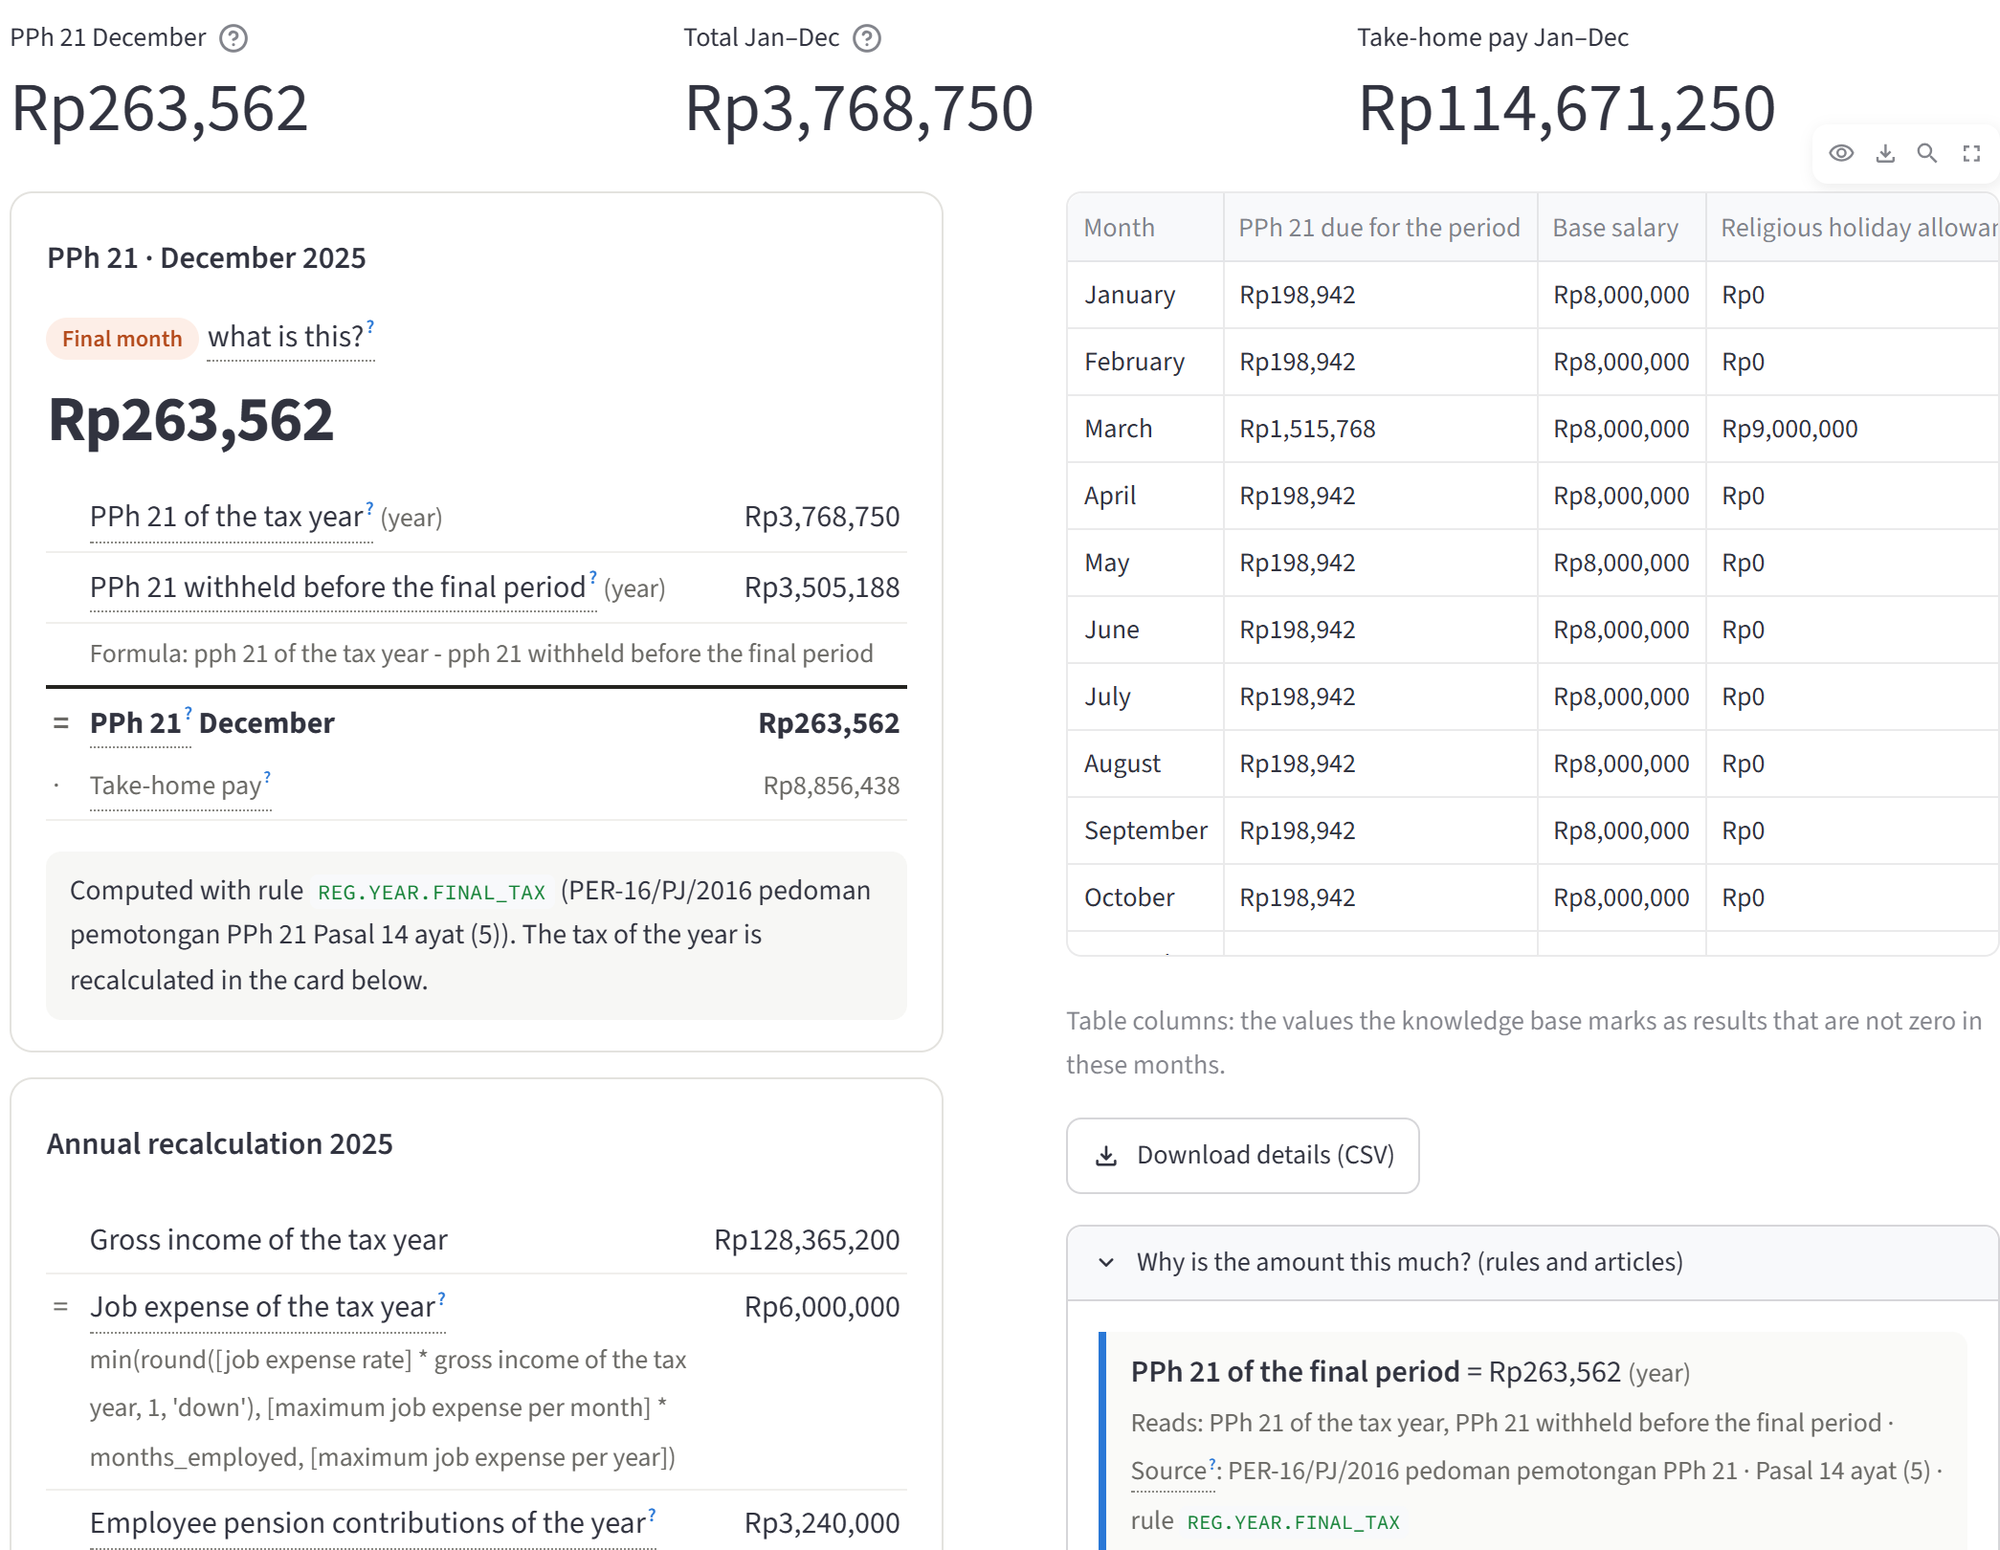
\includegraphics[width=0.9\textwidth]{figs/screen_calculator.png}
\caption{PPh 21 calculator of the application with the result of the final month and its rule.}
\label{fig:calc}
\end{figure*}

A retroactive rule needs no special code even when its update is recorded on date $\omega_1$ after a payroll has run on the knowledge of $\omega_0 < \omega_1$. The recalculation report then evaluates each employee at both knowledge dates and lists every value that differs in the months already paid. The employer receives the correction per employee and month. The payroll as computed on $\omega_0$ remains reproducible because no record is overwritten.

\subsection{LLM-Assisted Update Pipeline}
\label{sec:acquisition}
The update pipeline turns one document into at most one proposed update (Fig.~\ref{fig:acqflow}). It locks the document text with SHA-256 and splits it into parts by article. A low-cost model first maps each part as core (sent word for word), general (sent as a summary), or none (left out). Core parts are never cut. A drafting model then judges whether the document changes the PPh 21 computation and must support its judgment with verbatim quotes. A document judged not relevant ends with an empty update. For a relevant document, the drafting model writes three independent drafts of the update as structured JSON. Each draft lists the elements to add, change, or remove with a quote from the provision of each element. The prompt carries the vocabulary of facts and functions, the payroll data dictionary of the company, and the related records of the knowledge base retrieved with SPARQL. The model never computes tax.

\begin{figure*}[!t]
\centering
\figAcquisitionFlow
\caption{Update pipeline for one document.}
\label{fig:acqflow}
\end{figure*}

Six deterministic gates check every draft in the order of Table~\ref{tab:gates} and stop at the first failure. The static checks run first because G4 and G5 must execute the engine on generated cases. G6 is static and therefore runs second although it is numbered last. G1 applies the JSON schema, the application of the update to the knowledge base, and the SHACL shapes. G6 requires every case-data input that a new rule reads to exist in the payroll data of the company. Without this gate, a draft could invent an input such as an employee attribute that the generated test cases supply but real payroll data never contains. G2 requires each quote to occur in the document and every new number and date to occur in the quote of its element. G3 checks expressions, the dependency graph, and references. G4 runs the knowledge base before and after the update on a set $\SG$ of up to 300 cases generated from the draft and rejects new engine errors and changes before the start of validity.

The set $\SG$ combines PTKP statuses, withholding methods, salary levels, and the thresholds of the changed elements and is filled with random combinations to about 250 cases. It is generated from the draft alone and never reads the reference knowledge base or the test cases. G5 reports elements that change no output on $\SG$ to the reviewer without rejecting the draft. A draft that fails receives the gate messages and one repair round. Among the 354 drafts of the isolated runs, 151 failed a gate at first, and 31 of them passed after the repair round. A completeness gate G7 was defined after the evaluation and is reported separately in Section~\ref{sec:res-gate}.

\begin{table}[!t]
\caption{Verification gates and the first gate that failed among the 354 drafts of the isolated runs.}
\label{tab:gates}
\centering\footnotesize
\setlength{\tabcolsep}{3pt}
\begin{tabularx}{\columnwidth}{@{}lLLr@{}}
\toprule
Gate & Checks & Example of a failure & Drafts \\
\midrule
G1 & schema, application, SHACL & a missing required validity date or an annex table that was not extracted & 39 \\
G6 & inputs exist in payroll data & a rule reading an invented attribute for head-office staff & 96 \\
G2 & quotes, numbers, dates & an end of validity that no quote supports & 9 \\
G3 & expressions, references & a rule reading a table that is not yet valid & 2 \\
G4 & regression on $\SG$ & a tax facility that changes months before its start of validity & 5 \\
G5 & effect of each element & reported to the reviewer & 0 \\
\bottomrule
\end{tabularx}
\end{table}

The drafts that pass are grouped by their behavior on the union of their $\SG$ sets at the day before and the day of issue. Two drafts belong to the same group when they give the same output values, conflict report, and engine errors on every case of this union at both dates. The first draft of the largest group in a random order becomes the proposal. A single passing draft forms the largest group on its own. A tie or the absence of a passing draft ends in abstention, which sends the document to the HC software engineer without a proposal.

\subsection{Review by an HC Software Engineer}
\label{sec:review}
The intended reviewer is an HC software engineer of the human capital division. This engineer builds and maintains the company's human capital information system (HCIS) with its payroll module and can therefore read both the payroll data and the rules. The role exists in companies that develop their own HCIS. The review page shows the proposal with its quotes, the gate results, before-and-after payslips for a fixed set of payroll scenarios, and the company policies whose rules read a fact that the update touches. The engineer approves, edits, or rejects the proposal or asks the model to repair it. After an abstention the engineer writes the update. In both cases the engineer handles a structured change with its sources instead of writing new program code.

The application covers the upload of a document and the review of its proposal (Fig.~\ref{fig:manage}). A document is uploaded with its title, issue date, and type and waits on its card until the update pipeline is run. The review page lists the proposed changes with their quotes, the gate results, and the before-and-after results of the standard scenarios. The proposal in the figure was written by hand for illustration. The checks on this proposal report that its source document is not in the knowledge base.

\begin{figure*}[!t]
\centering
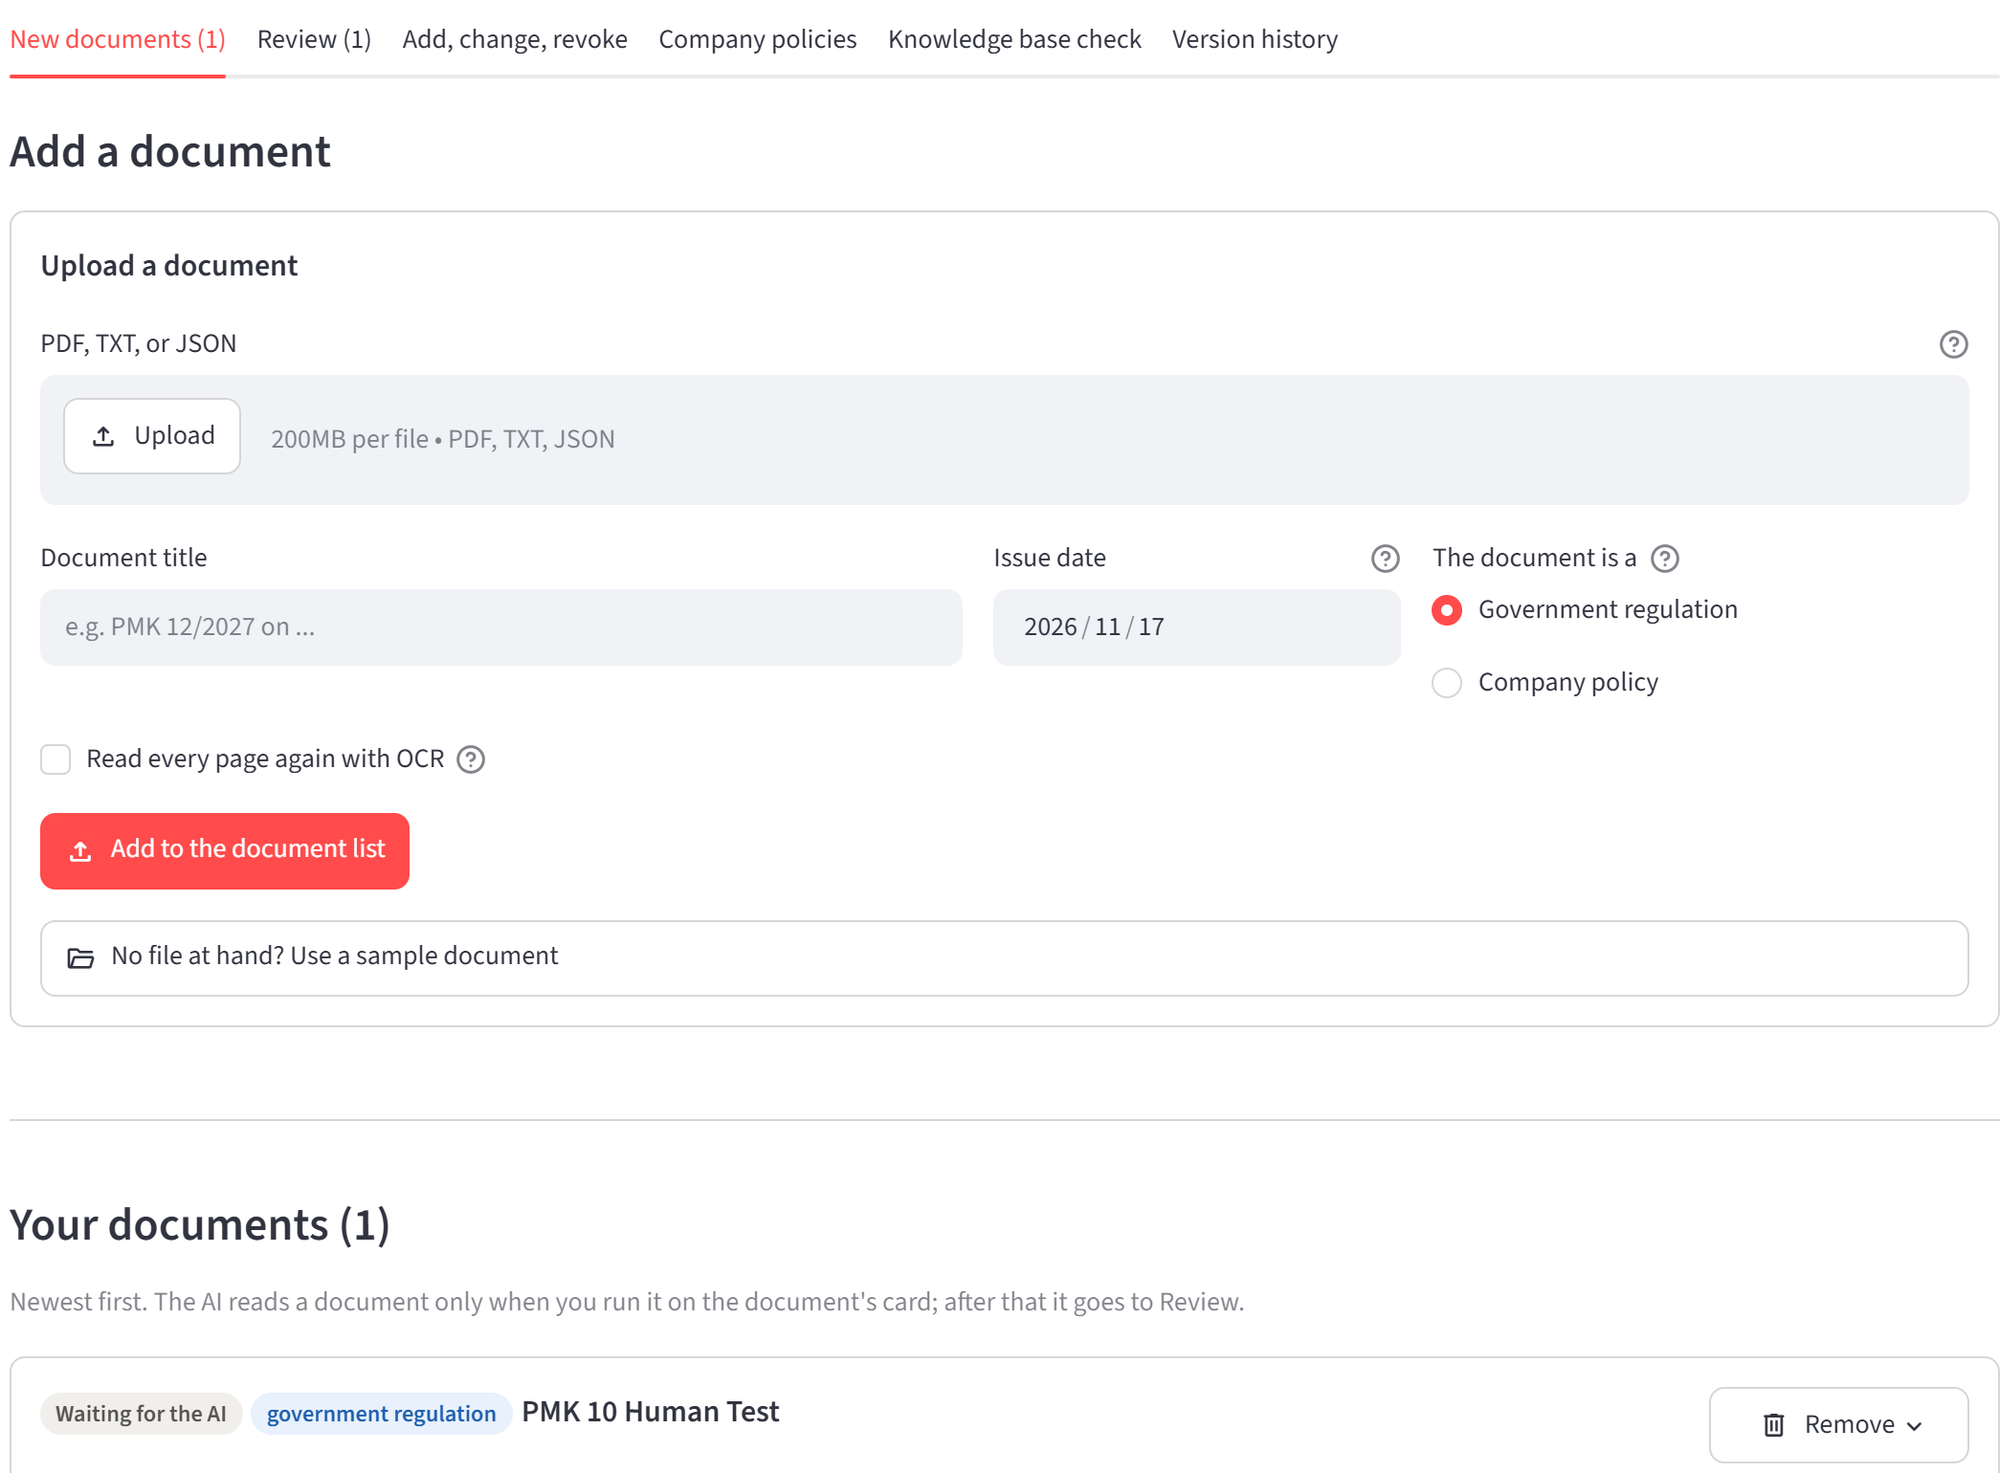
\includegraphics[width=0.6\textwidth]{figs/screen_upload.png}\\[1pt]{\footnotesize (a)}\\[4pt]
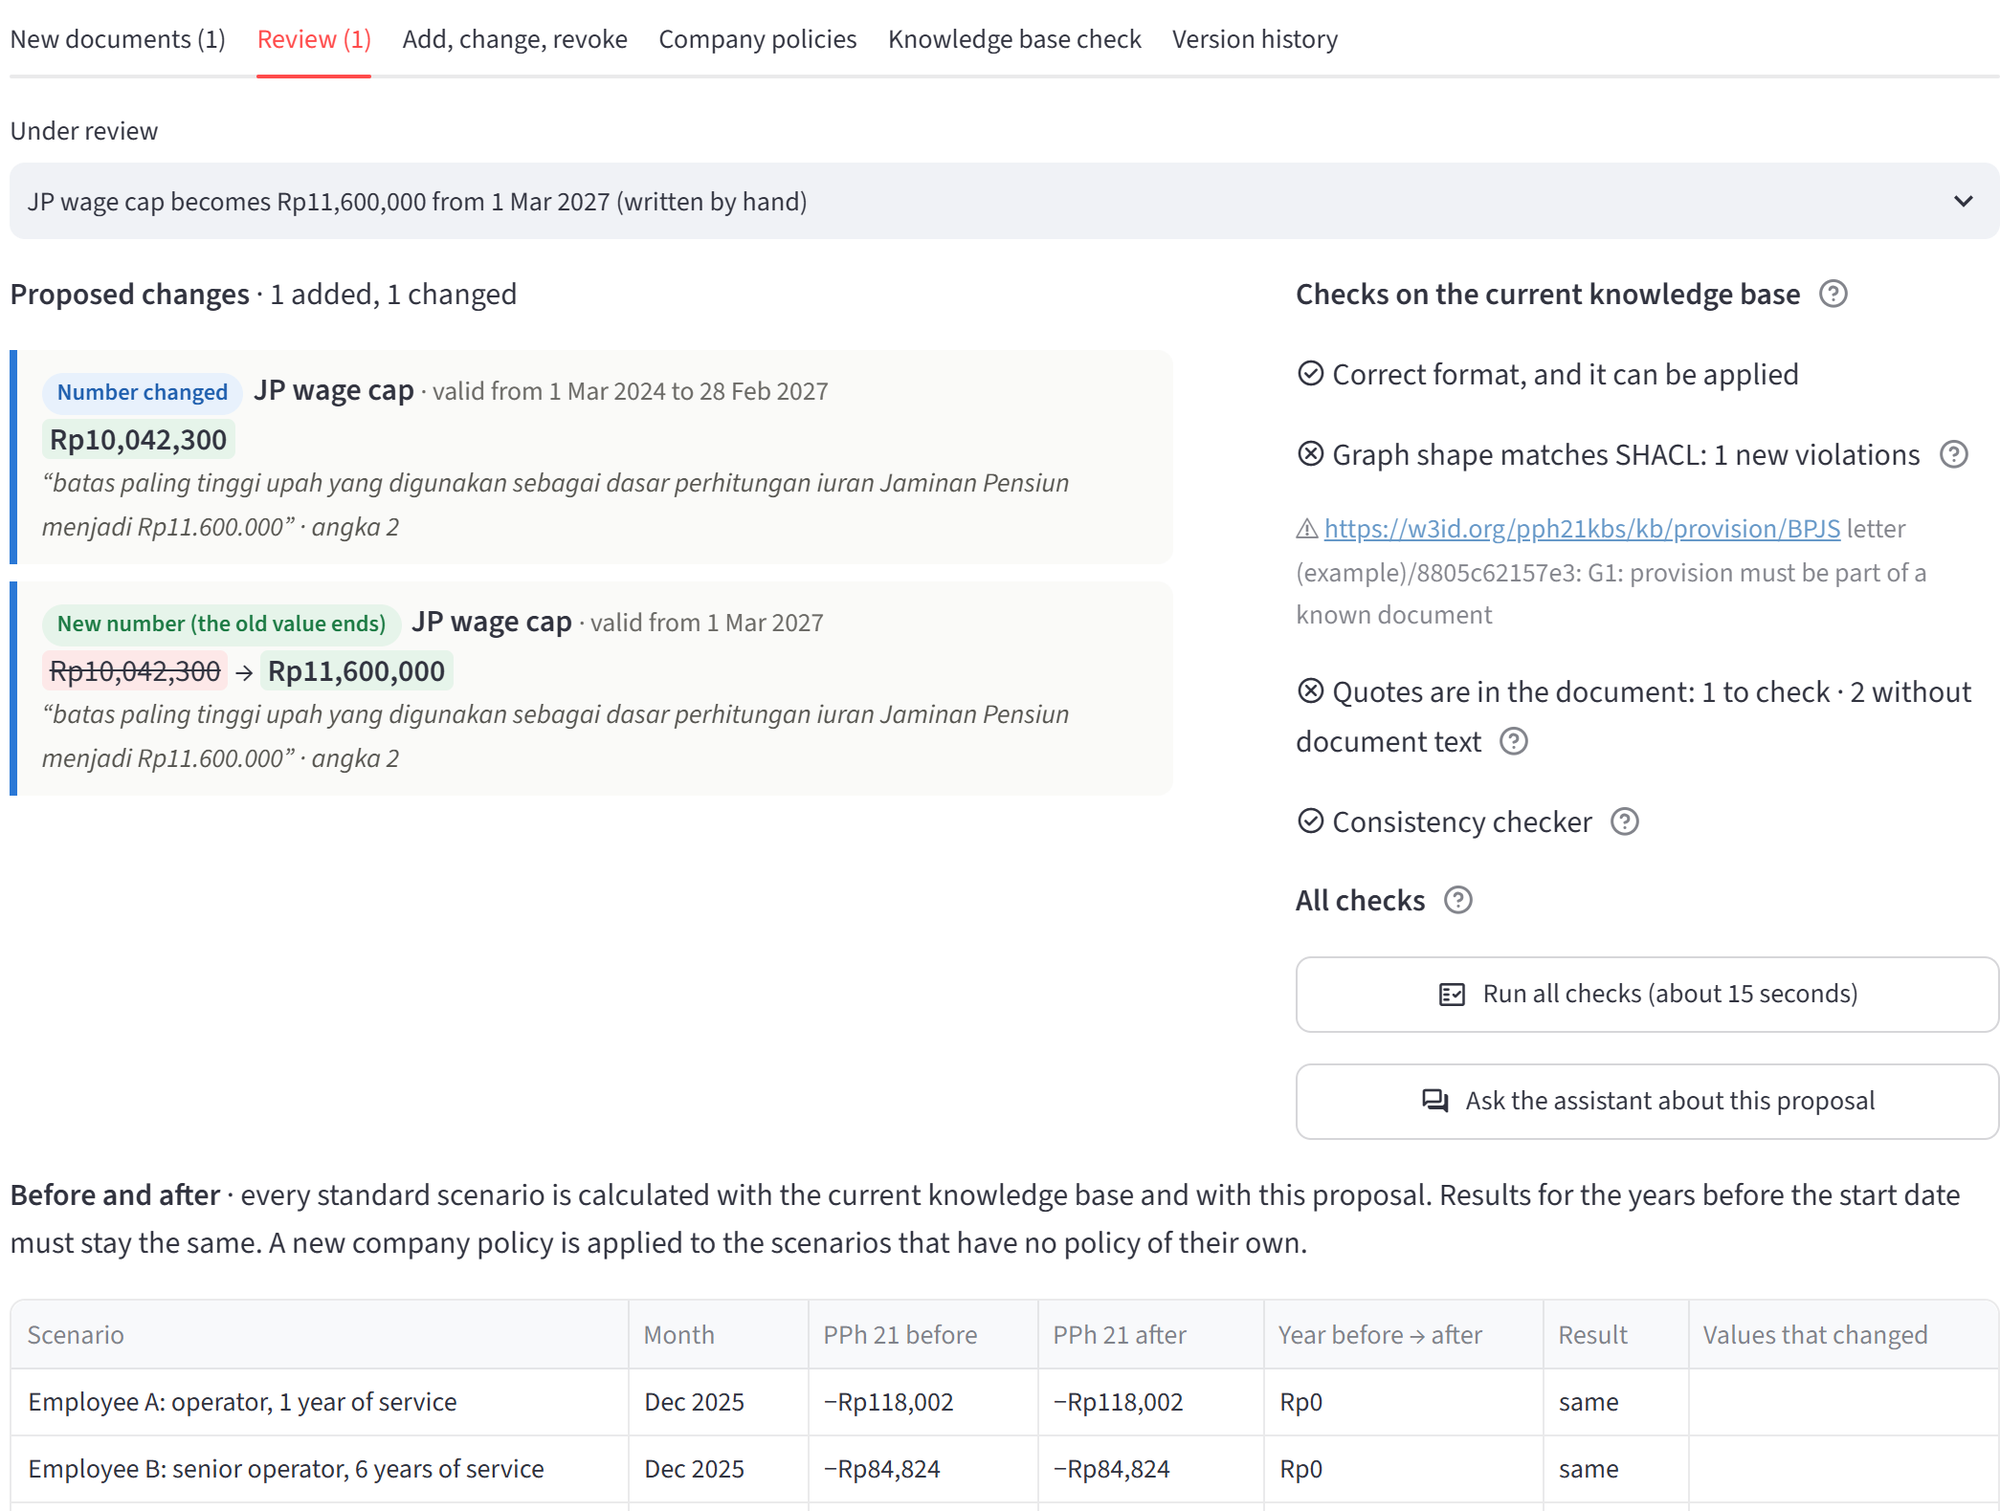
\includegraphics[width=0.6\textwidth]{figs/screen_review.png}\\[1pt]{\footnotesize (b)}
\caption{Knowledge base management with (a) the upload of a document and (b) the review of a proposal.}
\label{fig:manage}
\end{figure*}
